\chapter{Domain Driven Design}\label{chapter:domain_driven_design}

\section{Introduction}\label{section:domain_driven_design/introduction}
Understanding the problem space can be a very useful way to design software. The common way to understand the problem and communicate them is by using various design models. The design models are the abstraction as well as representation of the problem space. However, when the abstractions are created, there are chances that important concepts or data are ignored or misread. This will highly impact the quality of software produced. The software thus developed may not reflect the real world situation or problem entirely.
\\
Domain Driven Design provides a way to represent the real world problem space so that all the important concepts and data from real world remains intact in the model. The domain model thus captured respects the differences as well as the agreement in the concepts across various parts of the problem space. Moreover, it also provides a way to divide the problem space into manageable independent partitions and makes it easy for developers as well as stakeholders to focus on the area of concern as well as be more agile. Finally, the domain models act as the understandable and common view of the business for both domain experts as well as the developers. This will make sure that the software developed using domain driven design will comply with business need.\cite{Evans:2003aa}\cite{Vernon:2013aa}
\\

\section{Process to Domain Driven Design}\label{section:domain_driven_design/process_to_domain_driven_design}
There are three basic parts to implement domain driven design:
\begin{enumerate}
\item{Ubiquitous Language}
\item{Strategical Design}
\item{Tactical Design}
\end{enumerate}
\\
As the focus is to describe the process of identifying microservice candidates, only the first two parts are relevant and will be focused in the later part of this chapter.
\subsection{Ubiquitous Language}\label{section:domain_driven_design/process_to_domain_driven_design/ubiquitous_language}
Ubiquitous Language is a common language agreed among domain experts and developers in a team. It is important to have a common understanding about the concepts of a business which is being developed and ubiquitous language is the way to assure that. Domain Experts understand the domain in terms of their own jargon and concept. It is difficult for a developer to understand them. Usually, developers translates those jargons into the terms they understand easily during desing and implementation. However along the way of translation, major domain concepts can get lost and the immediate value of the resulting solution might decrease tremendously. In order to prevent creation of such low valued solution, there should be a meet-in-the-middle approach to define common vocabularies and concepts understood by all domain experts as well as the developers. These common vocabularies and concepts make the core of the ubiquitous language.\cite{Evans:2003aa}\cite{Vernon:2013aa}
\\
Along with the common vocabulary and concepts, domain models provide backbone to create ubiquitous language. The models represents not only artifacts but also functionalities, rules and strategies. It is a way to express the common understanding in a visual form providing an easy tool to comprehend.\cite{Evans:2003aa}\cite{Fowler:2006aa} According to \cite{Fowler:2003aa}, domain model should not be confused with data model which represents the business in datacentric view but rather each domain object should contain data as well as logic closely related to the data contained. Domain models are conceptual models rather than software artifacts but can be effectively visualized using \acrshort{UML}.\cite{Scott:2001aa}

\begin{figure}[H]
\begin{center}
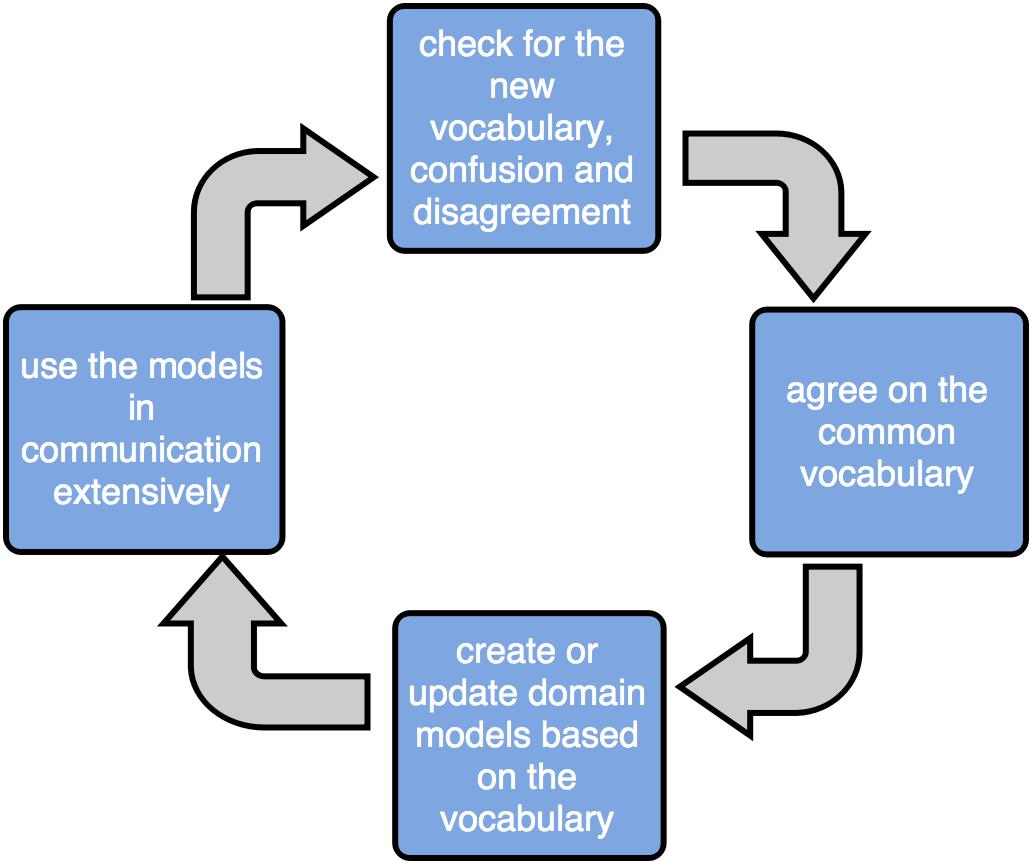
\includegraphics[width=0.8\textwidth]{figures/domain-driven-design-one}
\caption{Process to define Ubiquitous Language \cite{Evans:2003aa}}
\label{fig:domain_driven_design/ubiquitous_language_process}
\end{center}
\end{figure}
\\
The figure \ref{fig:domain_driven_design/ubiquitous_language_process} visualizes the process of discovering the ubiquitous language in any domain. It is not a discretely timed phenomenon but a continous procedure with various phases occuring in a cycle throughout the development.
\\
On arrival of any new term, concept or any confusion, the contextual meaning of those terms are made clear before adding to the domain vocabulary. Next, the vocabularies and concepts are used to create various domain models following \acrshort{UML}. The domain models and various vocabularies for the common laguage among domain experts and developers within the team. It is very important to use only domain vocabularies for communication and understanding which will not only help to reflect the hidden domain concepts in the implementation but also create opportunities to create new vocabularies or refine existing ones in the event of confusion and disagreement.\cite{Evans:2003aa}
\\
Thus, the common vocabulary and domain models form the core of the ubiquitous language and the only way of coming up with the better one is by applying it in communication extensively. Ubiquitous language is not just a collection or documentation of terms but is the approach of communication within a domain.
\\
\subsection{Strategical Design}\label{section:domain_driven_design/process_to_domain_driven_design/strategical_design}
When applying model-driven approach to an entire enterprise, the domain models get too large and complicated. It becomes difficult to analyse and understand all at once. Furthermore, it gets worse as the system gets bigger. The strategical design provides a way to divide the entire domain models into small,manageable and interoperable parts which can work together with low dependency in order to reflect the functionalities of the entire domain. The goal is to divide the system into modular parts which can be easily integrated. Additionally, the all-cohesive unified domain models of the entire enterprise cannot reflect differences in contextual vocabularies and concepts.\cite{Fowler:2014ab}\cite{Evans:2003aa}\cite{Vernon:2013aa}
\\
The strategical design specifies two major steps which are crucial in identifying microservices.
\\
\begin{shaded}Step 1: Divide problem domain into subdomains \end{shaded} \label{section:domain_driven_design/process_to_domain_driven_design/strategical_design/step_1}
\\
The domain represents the problem being solved by the software. The domain can be divided into various sub-domains based on the organizational structure of the enterprise, each sub-domain responsible for certain area of the problem. The \cite{Engels:2015aa} provides a comprehensive set of steps to identify sub-domains.
\begin{enumerate}
\item \textbf{Identify core business functionalities and map them into domain:} \\
A core business functionality represents the direct business capability which holds high importance and should be provided by the enterprise in order for it to succeed. For example, for any general e-commerce enterprise, the core focus will on the high amount orders being received from the customers and maintain the inventory to fulfil the orders. So, for those kind of e-commerce enterprises, 'Order Management' and 'Inventory Management' will be the some of the core domains.
\\
\item \textbf{Identify generic and supporting subdomains:} \\
The business capabilities which are viable for the success of business but not represent the specialization of the enterprise falls into supporting subdomains. The supporting subdomain does not require the enterprise to excel in these areas. Additionally, if the functionalities are not specific to the business but in a way support the business functionalities, then these are covered by generic subdomains. For example: for an e-commerce enterprise, 'Payment Management' can be a supporting subdomain whereas 'Reporting' and 'Authentication' can be generic subdomains.\cite{Vernon:2013aa}
\\
\item \textbf{Divide existing subdomains having multiple independent strategies:}\\
The subdomains found from earlier steps are analyzed to check if there are mutually independent strategies to handle the same functionality. The subdomain can then be further divided into multiple subdomains along the dimension of strategies. For example: the 'Payment Managment' subdomain discovered in earlier step can have different way of handling online payment depending upon the provider such as bank or paypal etc. In that case 'Payment Management' can be further divided into 'Bank Payment Management' and 'Paypal Payment Management'.
\end{enumerate}
\\
\begin{shaded}Step 2: Indentify bounded contexts\end{shaded} \label{section:domain_driven_design/process_to_domain_driven_design/strategical_design/step_2}
\\
As stated earlier of this section, the attempt to use a single set of domain models for the entire enterprise adds complexity for understanding and analysis. There is another important reason supporting the issue which is called unification of the domain models. Unification represents internal consistency of the terms and concepts described by the domain models. It is not always possible to have consistent meaning of terms without any contradictory rules throughout the enterprise. The identification of the logically consistent and inconsistent domain model creates a boundary around domain model. This boundary will bind all the terms which share consistent logic from those which are different from them so that there is clear understanding of the concept inside the boundary without any confusion. The shared context inside the boundary is defined as the bounded context.
\\
\textbf{Definition 1:} \label{bounded_context_definition_1}
\\
" A Bounded Context delimits the applicability of a particular model so that team members hava a clear and shared understanding of what has to be consistent and how it relates to other contexts. A bounded context has specific functionality and explicitly defines boundary around team organization, code bases and database schemas."\cite{Evans:2003aa}
\\
\textbf{Definition 2:} \label{bounded_context_definition_2}
\\
" A Bounded Context is an explicit boundary within which a domain model exists. Inside the boundary all terms and phrases of the Ubiquitous Language have specific meaning, and the model reflects the Language with exactness." \cite{Vernon:2013aa}
\\
\textbf{Definition 3:} \label{bounded_context_definition_3}
" A Bounded Context is a specific responsibility enforced by explicit boundaries." \cite{Mike:2012aa}
\\
Thus, the idea of bounded context provide the applicability of the ubiquitous language inside its boundary performing a specific responsibility. Outside the bounded contexts, teams have different ubiquitous language with different terms, concepts, meanings and functionalities. Apart from identifying independent and specific responsibilities inside a subdomain in order to identify bounded contexts, there are some general rules which can be considered as well.
\begin{enumerate}
\item \textbf{Assign individual bounded context to the subdomains identified in Step 1}
\\
Each subdomains have distinct functionalities and complete set of independent domain models to accomplish the functionalities. Thus, one to one mapping of subdomain and bounded context is possible ideally whereas in real cases, it may not be always possible which can be tackled using the rules discussed in further steps. For example: Order Management and Inventory Management can be two distinct bounded context each with own consistent ubiquitous language. \cite{Fowler:2014ab}\cite{Gorodinski:2013aa}
\\
\item \textbf{Identify polysemes}
\\
Polysemes are the terms which have different meaning in separate contexts. If the example of the generic subdomain 'Authentication' is taken. It can have an model 'Account' however the same model can refer to multiple concept such as social account identified by e-mail or registered account identified by unique username. The handling of these two separate concepts is also different which clearly suggests two separate context for each within 'Authentication' subdomain. Additionally, there can be polysemes in two separate domains as well. For example: there is also 'Account' model to identify bank account in the subdomain 'Bank Payment Management'. The identification of polysemes is vital to create clear boundary around which the concept and handling of such polysemes are consistent. \cite{Fowler:2014ab}
\\
\item \textbf{Identify independent generic functionality supporting the subdomain}
\\
There can be a necessity of independent technical functionality required to accomplish the business functionality of the subdomain only. Since it is only required by the particular subdomain, the functionality cannot be nominated as a generic subdomain. In such a case, the independent technical functionality can be realized as a separate bounded context. For example, in the subdomain 'Inventory Management', the functionality of full-text search can be assigned a separate bounded context as it is independent.\cite{Gorodinski:2013aa}
\end{enumerate}
\\
\section{Microservices and Bounded Context}\label{section:domain_driven_design/microservices_and_bounded_context}
Analyzing various definitions of microservices provided in section \ref{section:context/microservices_architecture_style}, a list of important features with respect to specific category such as granularity or quality was compiled in the table \ref{tab:context/microservices_architecture_style/keywords_extracted_from_various_definitions_of_microservice}. In addition to the definitions of bounded context provided in section \ref{bounded_context_definition_1}, the following definition of Domain Driven Design can be helpful to find analogy between a microservice and a bounded context.
\begin{shaded}Definition: Domain Driven Design\end{shaded}
"Domain Driven Design is about explaining what your company does in isolated parts, in performing these specific parts and you can have a dedicated team to do this stuff, and you can have different tools for different teams." \cite{Riggins:2015aa}
\\
\\
Using table \ref{tab:context/microservices_architecture_style/keywords_extracted_from_various_definitions_of_microservice} and concepts extracted from various definitions of bounded context as well as Domain Driven Design provided, the table \ref{tab:domain_driven_design/microservices_and_bounded_context/Analogy_of_Microservice_and_Bounded_Context} is generated. 
\\
\begin{table}[h!]
  \centering
  \begin{adjustbox}{max width=\textwidth}
  \begin{tabular}{*{14}{|c}|}%%{|c|c|}
  \hline
  \# & Expected features of a microservice  & Fulfilled by Bounded Context\\
  \hline
  \hline
   1 & Loosely coupled, related functions           & \checkmark  \\ \hline
   2 & Developed and deployed independently       & \checkmark \\ \hline
   3 & Own database                                 & \checkmark \\ \hline
   4 & Different database technologies         & \checkmark  \\ \hline
   5 & Build around Business Capabilities  & \checkmark\\ \hline
   6 & Different Programming Languages & \checkmark \\ \hline
   \hline
   \end{tabular}
\end{adjustbox}
  \caption{Analogy of Microservice and Bounded Context}
  \label{tab:domain_driven_design/microservices_and_bounded_context/Analogy_of_Microservice_and_Bounded_Context}
\end{table}
\\
The table \ref{tab:domain_driven_design/microservices_and_bounded_context/Analogy_of_Microservice_and_Bounded_Context} lists various features expected by a microservices. Again, it shows that the tabulated features are fulfilled by a bounded context. It can be implied that a microservice is conceptually analogous to a bounded context. The section \ref{section:domain_driven_design/process_to_domain_driven_design} provided the detailed process to discover bounded contexts within a large domain, which ultimately also provides guidelines to determine microservices using domain driven design principles.
\\
Furthermore, there can be found enough evidence regarding the analogy as well as practical implementation of the concept. The table lists various articles which agree on the analogy and in most cases, have utilized the concepts to create microservices in real world.
\begin{table}[h!]
  \centering
  \begin{adjustbox}{max width=\textwidth}
  \begin{tabular}{*{14}{|c}|}%%{|c|c|}
  \hline
  \# & Articles  & Agreement on the Concept & Utilized Bounded Context to create Microservices\\
  \hline
  \hline
   1 & \cite{Mauro:2015aa}           & \checkmark & \checkmark  \\ \hline
   2 & \cite{Hughson:2014aa}       & \checkmark & \\ \hline
   3 & \cite{Fowler:2014aa}        & \checkmark & \\ \hline
   4 & \cite{Sokhan:2015aa}       & \checkmark  & \\ \hline
   5 & \cite{Daya:2015aa}   & \checkmark & \checkmark \\ \hline
   6 & \cite{Riggins:2015aa} & \checkmark & \\ \hline
   7 & \cite{Beard:2015aa} & \checkmark  & \checkmark \\ \hline
   8 & \cite{Krylovskiy:2015aa} & \checkmark  & \checkmark \\ \hline
   9 & \cite{Viennot:2015aa} & \checkmark  & \checkmark \\ \hline
   10 & \cite{Balalaie:2015aa} & \checkmark  & \checkmark \\ \hline
   \hline
   \end{tabular}
\end{adjustbox}
  \caption{Application of Bounded Context to create Microservices}
  \label{tab:domain_driven_design/microservices_and_bounded_context/Microservices_following_Bounded_Context}
\end{table}
\\

\section{Example Scenario}\label{section:domain_driven_design/example_scenario}
In this section, a case study will be discussed. The case study will be used to design the system using microservices architecture following the domain driven design given supported by the section \ref{section:domain_driven_design/process_to_domain_driven_design}.

\begin{shaded} Case Study \end{shaded} \label{section:domain_driven_design/example_scenario/case_study}
The case study is for the same hotel introduced in the section \ref{section:selection_by_use_case/refactoring_example}. The hotel 'XYZ' is thinking of upgrading its current system and adding new business usecases in order to tune its competitive edge in the market.\\
Previously, the hotel only supported booking of the rooms, payment by cash, cancelation of booking and finally viewing of the room details.\\
The hotel has planned to provide various package offerings to the either general customers or specific group of customers satisfying certain profile. Firstly, a hotel staff creates a package with name, description, valid time period, applicable type of room and location and discount associated with the package. Furthermore, the package will also contain certain constraints such as maximum number of offerings and maximum number of offerings per customer. The offering is represented by coupon and has unique identity. Once a package is created, the package has to be activated either by the hotel staff or by the activation time trigger. Only, the activated packages are visible to the customers. The customers can apply for the active packages. The customer profile is validated against the expected profile for the package and then a new coupon is sent to the customer.\\
The room booking workflow has no changes from the old system where a customer can view list of rooms with various information and send room booking request to the system. The system will then send confirmation with unique booking code to the customer.\\
Finally, the payment can be done by debit card or by paypal. During the payment, the customer can specify a valid coupon. The payment system will then redeem the coupon so that the respective discount represented by the coupon is deducted from the overal price.\\
Additionally, a detailed report is planned to be made available for customers showing various transactions with the hotel for the room bookings along with the information of the rooms till date. Similarly, hotel staff has various types of reports such as profit statement and room booking status.\\
The steps listed in \ref{section:domain_driven_design/process_to_domain_driven_design} can be used to design the system defined by the case study \ref{section:domain_driven_design/example_scenario/case_study}.
\textbf{\underline{Step 1:}}
\\
With reference to the steps shown by the figure \ref{fig:domain_driven_design/ubiquitous_language_process}, the first step would be to find out new domain vocabularies, understand the meaning, agree on them and use them as the common vocabularies. The table \ref{tab:domain_driven_design/example_scenario/domain_keywords} lists some important domain terms taken from the case study \ref{section:domain_driven_design/example_scenario/case_study} and clarifies the meaning for each. It is interesting to notice that the term 'Profile' has two different meaning depending upon the context of package and customer and it is a polyseme.
\begin{table}[H]
  \centering
  \begin{adjustbox}{max width=\textwidth}
  \begin{tabular}{*{14}{|c}|}%%{|c|l|}
  \hline
  \textbf{Domain Terms} & \textbf{Definition} \\
  \hline
  Package & a discount offering to certain group of customers\\ \hline
  Profile & the expected characteristics of customers to be elligible to apply a package\\ \hline
  Discount & the reduction value offered in the total price for hotel service\\ \hline
  Constraint & defines the limitation of creating coupons for any package\\ \hline
  Coupon & represents the authorized assignment of a valid package to a valid customer, which can be used later\\ \hline
  Customer Profile & the current characteristics of a customer\\ \hline
  Room Booking & assignment of a room to a customer for certain period\\ \hline
  Booking Code & a unique code representing the valid room booking\\ \hline
  Redeem Coupon & request to use the coupon whereby the associated discount value is deducted from the total price\\ \hline
  Price & the total amount for the hotel service\\ \hline
\end{tabular}
\end{adjustbox}
  \caption{Domain Keywords}
  \label{tab:domain_driven_design/example_scenario/domain_keywords}
\end{table}
\\

\textbf{\underline{Step 2:}}
\\
Next, the subdomains are identified following the step 1 \ref{section:domain_driven_design/process_to_domain_driven_design/strategical_design/step_1} of strategical design. The core domains, supporting domains and generic domains are identified and listed in the table.
\\
\\
\begin{table}[H]
  \centering
  \begin{adjustbox}{max width=\textwidth}
  \begin{tabular}{*{14}{|c}|}%%{|c|l|}
  \hline
  \textbf{Core Domains} & 
                    \begin{tabular}{ll}
                    \multirow{3}{*}
                    & 1 Package\\
                    & 2 Booking\\
                    & 3 Checkout\\
                    \end{tabular}\\
                    \hline
                    
   \textbf{Supporting Domains} &
                    \begin{tabular}{ll}
                    \multirow{3}{*}
                    &
                    \begin{tabular}{ll}
                    \multirow{2}{*}{1 Payment}
                    & 1.1 Paypal\\
                    & 1.2 CardPayment\\
                    \end{tabular}\\
                    & 
                    \begin{tabular}{ll}
                    \multirow{2}{*}{2 User Management}
                    & 2.1 Customer Management\\
                    & 2.2 Staff Management\\
                    \end{tabular}\\
                    & 3 Room\\
                    \end{tabular}\\
                    \hline
                    
    \textbf{Generic Domains} &
                    \begin{tabular}{ll}
                    \multirow{2}{*}
                    & 1 Reporting\\
                    & 2 Authentication\\
                    \end{tabular}\\
                    \hline
\end{tabular}
\end{adjustbox}
  \caption{Subdomains}
  \label{tab:domain_driven_design/example_scenario/subdomains}
\end{table}
\\

The supporting domain "User Management" has different stragegy for Customer and Staff so can be further divided into "Customer Management" and "Staff Management" subdomains. For the same reason, the "Payment" subdomain can also be further divided into "Paypal" and "CardPayment".
\\
\textbf{\underline{Step 3:}}
\\
The next action is to identify bounded context following the process described in step \ref{section:domain_driven_design/process_to_domain_driven_design/strategical_design/step_2}. The process is implemented in each subdomains. In order to accomplish this, domain models can be constructed for each subdomain. Along the process, the various ambguities in the domain models and clear understanding of the concept of the models can be clarified. This will highly help to achieve consistent ubiquitious language with the unification of domain models as well as shared vocabulary inside each subdomain. The boundary around the uniform and consistent domain represents the bounded contexts. Additionally, the rules given in the section \ref{section:domain_driven_design/process_to_domain_driven_design/strategical_design/step_2} can be applied when appropriate to identify bounded contexts.
The following section will provide the analysis of major subdomains to identify the bounded contexts within.\\
\begin{shaded} Customer Management \end{shaded}
\\
\begin{figure}[H]
\begin{center}
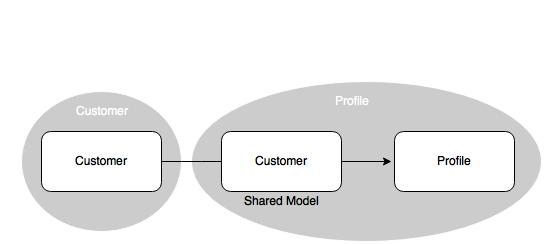
\includegraphics[width=0.8\textwidth]{figures/domain-driven-design-two}
\caption{Domain Model for Customer Management}
\label{fig:domain_driven_design/example_scenario/subdomains/Customer}
\end{center}
\end{figure}
\\
The management of customer includes two distinct broad task which are managing the customer itself and management of attributes of each customer which contribute to creating profile of customer at any point of time. Although, these two functionalities are related to customer, are actually loosely coupled and have different performance requirement. For eg: the change in the decision of adding attribute to a customer profile does not change the way customer is managed and also the rate at which customer profile is updated will definitely have high value than the rate customer is managed. Additionally, not all the attributes from customer is relevant to customer profile which makes 'Customer' a polyseme and a shared model between the two bounded contexts 'Customer' and 'Profile'.\\

\begin{shaded} Booking \end{shaded}
\\
\begin{figure}[H]
\begin{center}
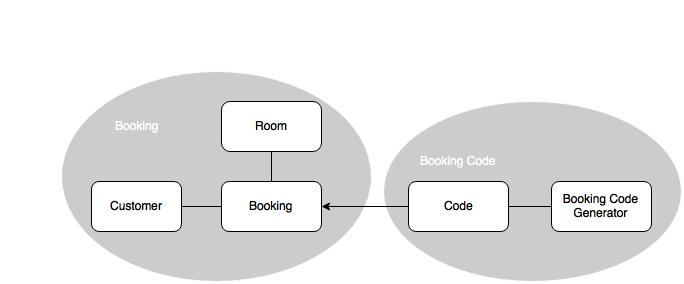
\includegraphics[width=0.8\textwidth]{figures/domain-driven-design-three}
\caption{Domain Model for Booking}
\label{fig:domain_driven_design/example_scenario/subdomains/booking}
\end{center}
\end{figure}
\\
The figure \ref{fig:domain_driven_design/example_scenario/subdomains/booking} shows the domain models of "Booking" subdomain. All the domain models and terms inside the subdomain are consistent and clear. However, the models 'Room', 'Customer', 'Booking' and 'Code' are closely related to booking functionality whereas the functionality of generating the booking code can be considered independent of booking. This gives two loosely coupled bounded contexts: "Booking" and "Booking Code". It is also interesting to notice that the models 'Customer' and 'Room' are polysemes with regard to other 'Customer' and 'Room' bounded contexts.\\
\begin{shaded} Checkout \end{shaded}
\\
\begin{figure}[H]
\begin{center}
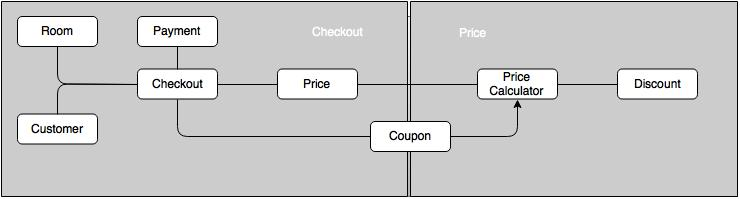
\includegraphics[width=0.8\textwidth]{figures/domain-driven-design-four}
\caption{Domain Model for Checkout}
\label{fig:domain_driven_design/example_scenario/subdomains/checkout}
\end{center}
\end{figure}
\\
The overall billing price calculation during checkout, which includes validation of coupon and redeem of the coupon onto the total price, is independent of the orchestration logic which occurs during checkout. The subdomain can be realized into two different bounded contexts 'Checkout' and 'Price'. Additionally, the domain models 'Customer, 'Discount', 'Room', 'coupon' and 'price' are polysemes for these bounded context with respect to other bounded contexts.\\
\begin{shaded} Package Management \end{shaded}
\\
\begin{figure}[H]
\begin{center}
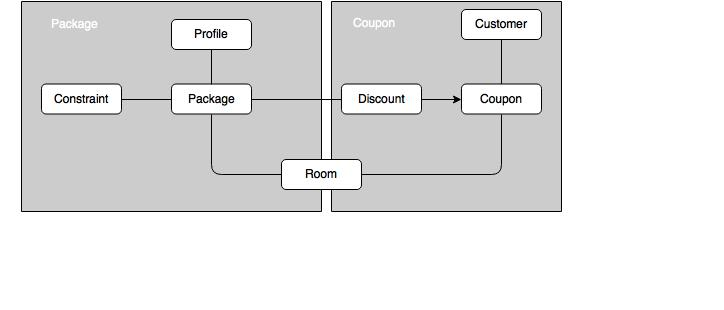
\includegraphics[width=0.8\textwidth]{figures/domain-driven-design-five}
\caption{Domain Model for Package Management}
\label{fig:domain_driven_design/example_scenario/subdomains/package-management}
\end{center}
\end{figure}
\\
The logic of package management can be considered independent of the way coupon is generated and validated. The packages are created by staff memeber whereas a coupon is created upon receiving a request from customer. Additionally, these are very specific and independent responsibilities, eligible of having own bounded contexts. The only data shared by the bounded contexts are about the information regarding eligible rooms and discount values. It should be made clear at this point that the 'Profile' domain model here is very different than 'Profile' domain model from 'Profile' boundend context of 'Customer Management' subdomain. In here, 'Profile' model defines the attributes of generic customer eligible for a specific package, however the 'Profile' domain model in 'Profile' bounded context provides the updated characteristics of any individual customer at the moment. Similarly, the models such as 'Customer' and 'Room' are polysemes.\\
The same process can be applied to identify bounded contexts for rest of the subdomains.